% Содержимое отчета по курсу Анализ алгоритмов

\aaunnumberedsection{ВВЕДЕНИЕ}{sec:intro}

Система конвейерной (потоковой) обработки данных --- система, состоящая из вычислительной и потребляющей частей, в которой задержка между отправкой и приёмом сообщений составляет порядка секунд--минут~\cite{streaming-data}.

Данная система хорошо согласуется с сервис-ориентированной архитектурой, при которой функциональность приложения представляется в виде набора слабо связанных автономных компонентов, называемых сервисами~\cite{services}.

Цель работы --- получение навыка организации параллельных вычислений по конвейерному принципу.

Задачи работы:
\begin{itemize}
    \item анализ предметной области;
    \item разработка алгоритма обработки данных;
    \item создание ПО, реализующего разработанный алгоритм;
    \item исследование характеристик созданного ПО.
\end{itemize}

\aasection{Входные и выходные данные}{sec:input-output}
Входными данными являются:
\begin{itemize}
	\item $URL$ начальной страницы;
	\item множество $URL$ начальных путей страниц, исключаемых из этапа обработки (может быть пустым);
	\item максимальное количество загружаемых страниц, где ноль обозначает отсутствие лимита.
\end{itemize}

Выходными данными являются загруженные в коллекцию СУБД $MongoDB$ $JSON$-документы, содержащие следующую информацию:
\begin{itemize}
	\item $id$ --- уникальный идентификатор рецепта;
	\item $issue\_id$ --- номер задачи из $Redmine$;
	\item $url$ --- $URL$ страницы рецепта;
	\item $title$ --- название рецепта;
	\item $ingredients$ --- массив ингредиентов, каждый ингредиент --- словарь вида (пример на $JSON$) \texttt{\{"name": название, "unit": единица измерения, "quantity": количество\}};
	\item $steps$ --- шаги рецепта, массив строк, одна строка --- одно предложение;
	\item $image\_url$ --- $URL$ основного изображения рецепта (если есть).
\end{itemize}

На рисунке~\ref{img:user-interface} представлен пример пользовательского интерфейса.

\aasection{Преобразование входных данных в выходные}{sec:algorithm}

На рисунке~\ref{img:architecture} изображена диаграмма архитектуры приложения.

\begin{figure}[!ht]
	\center{\includesvg[width=1\linewidth]{inc/img/architecture_diagram.svg}}
	\caption{Диаграмма архитектуры приложения}
	\label{img:architecture}
\end{figure}

Приложение включает в себя следующие сервисы:
\begin{itemize}
	\item $web$-сервер для получения, обработки и сохранения входных данных пользователя, сервис помещает в очередь новых ссылок первую задачу;
	\item $RabbitMQ$ --- брокер сообщений, обслуживающий очередь ссылок страниц, которые необходимо загрузить, также называемую $new\_links\_queue$, очередь новых страниц $new\_documents\_queue$, которые необходимо обработать и очередь новых рецептов $new\_recipes\_queue$, которые необходимо поместить в базу данных документов;
	\item $MongoDB$ --- предназначенная для работы с документами СУБД, хранящая обработанные рецепты в формате $JSON$;
	\item обслуживающий аппарат, загружающий страницы, также называемый $load\_automaton$. Сервис получает $URL$ из сообщения в очереди $new\_links\_queue$, загружает соответствующую $HTML$-страницу и помещает в очередь $new\_documents\_queue$ сообщение следующего формата \texttt{<url>:<html>}, где \texttt{<url>} и \texttt{<html>} --- $URL$ загруженной страницы и её текстовое представление, всё содержимое сообщение кодируется в формате $UTF-8$;
	\item обслуживающий аппарат, обрабатывающий страницы, также называемый $parse\_automaton$. Сервис получает $URL$ страницы и её $HTML$ наполнение. В результате обработки сервис извлекает множество ссылок, удовлетворяющих входным данным, и добавляет новые ссылки в очередь $new\_links\_queue$, при наличии на странице рецепта, извлекает его, помещает в соответствующую структуру, сериализует и помещает в очередь $new\_documents\_queue$;
	\item обслуживающий аппарат, сохраняющий рецепты, также называемый $store\_automaton$. Сервис получает сериализованную структуру-представление $JSON$ рецепта, десериализует её и помещает в базу данных $parsed\_recipes$ в коллекцию $recipes$ СУБД $MongoDB$.
	\item $Redis$ --- СУБД, хранящая множество обработанных ссылок для исключения их повторной обработки, целевой $URL$, с которым производится сравнение обрабатываемых ссылок (обрабатываемая ссылка не подлежит загрузке, если она не начинается с целевого $URL$), множество исключённых корневых $URL$ (обрабатываемая ссылка не подлежит загрузке, если она начинается хотя бы с одного исключённого $URL$), а также максимальное количество загружаемых страниц и текущее количество загруженных страниц.
	\item $InfluxDB2$ --- СУБД, предназначенная для работы с временными рядами. Данный сервис хранит временные метки событий, связанных с началом и концом обработки задачи обслуживающими аппаратами, а также временные метки поступления задачи в очередь обслуживающего аппарата, загружающего страницы.
	\item $Grafana$ --- $BI$-инструмент, позволяющий получить такую информацию, как среднее время обработки задачи отдельными обслуживающими аппаратами, среднее время ожидания задачи в каждой очереди и среднее время от начала до конца существования задачи. Перечисленная статистика доступна только для задач, прошедших через все обслуживающие аппараты, остальные задачи в статистике не учитываются.
\end{itemize}


\clearpage

На рисунках~\ref{img:sequence-diagram-pt-1}--\ref{img:sequence-diagram-pt-2} изображена диаграмма последовательности, визуализирующая пример взаимодействия сервисов системы при обработке первой страницы, содержащей 2 новые ссылки и рецепт.

\begin{figure}[!ht]
	\center{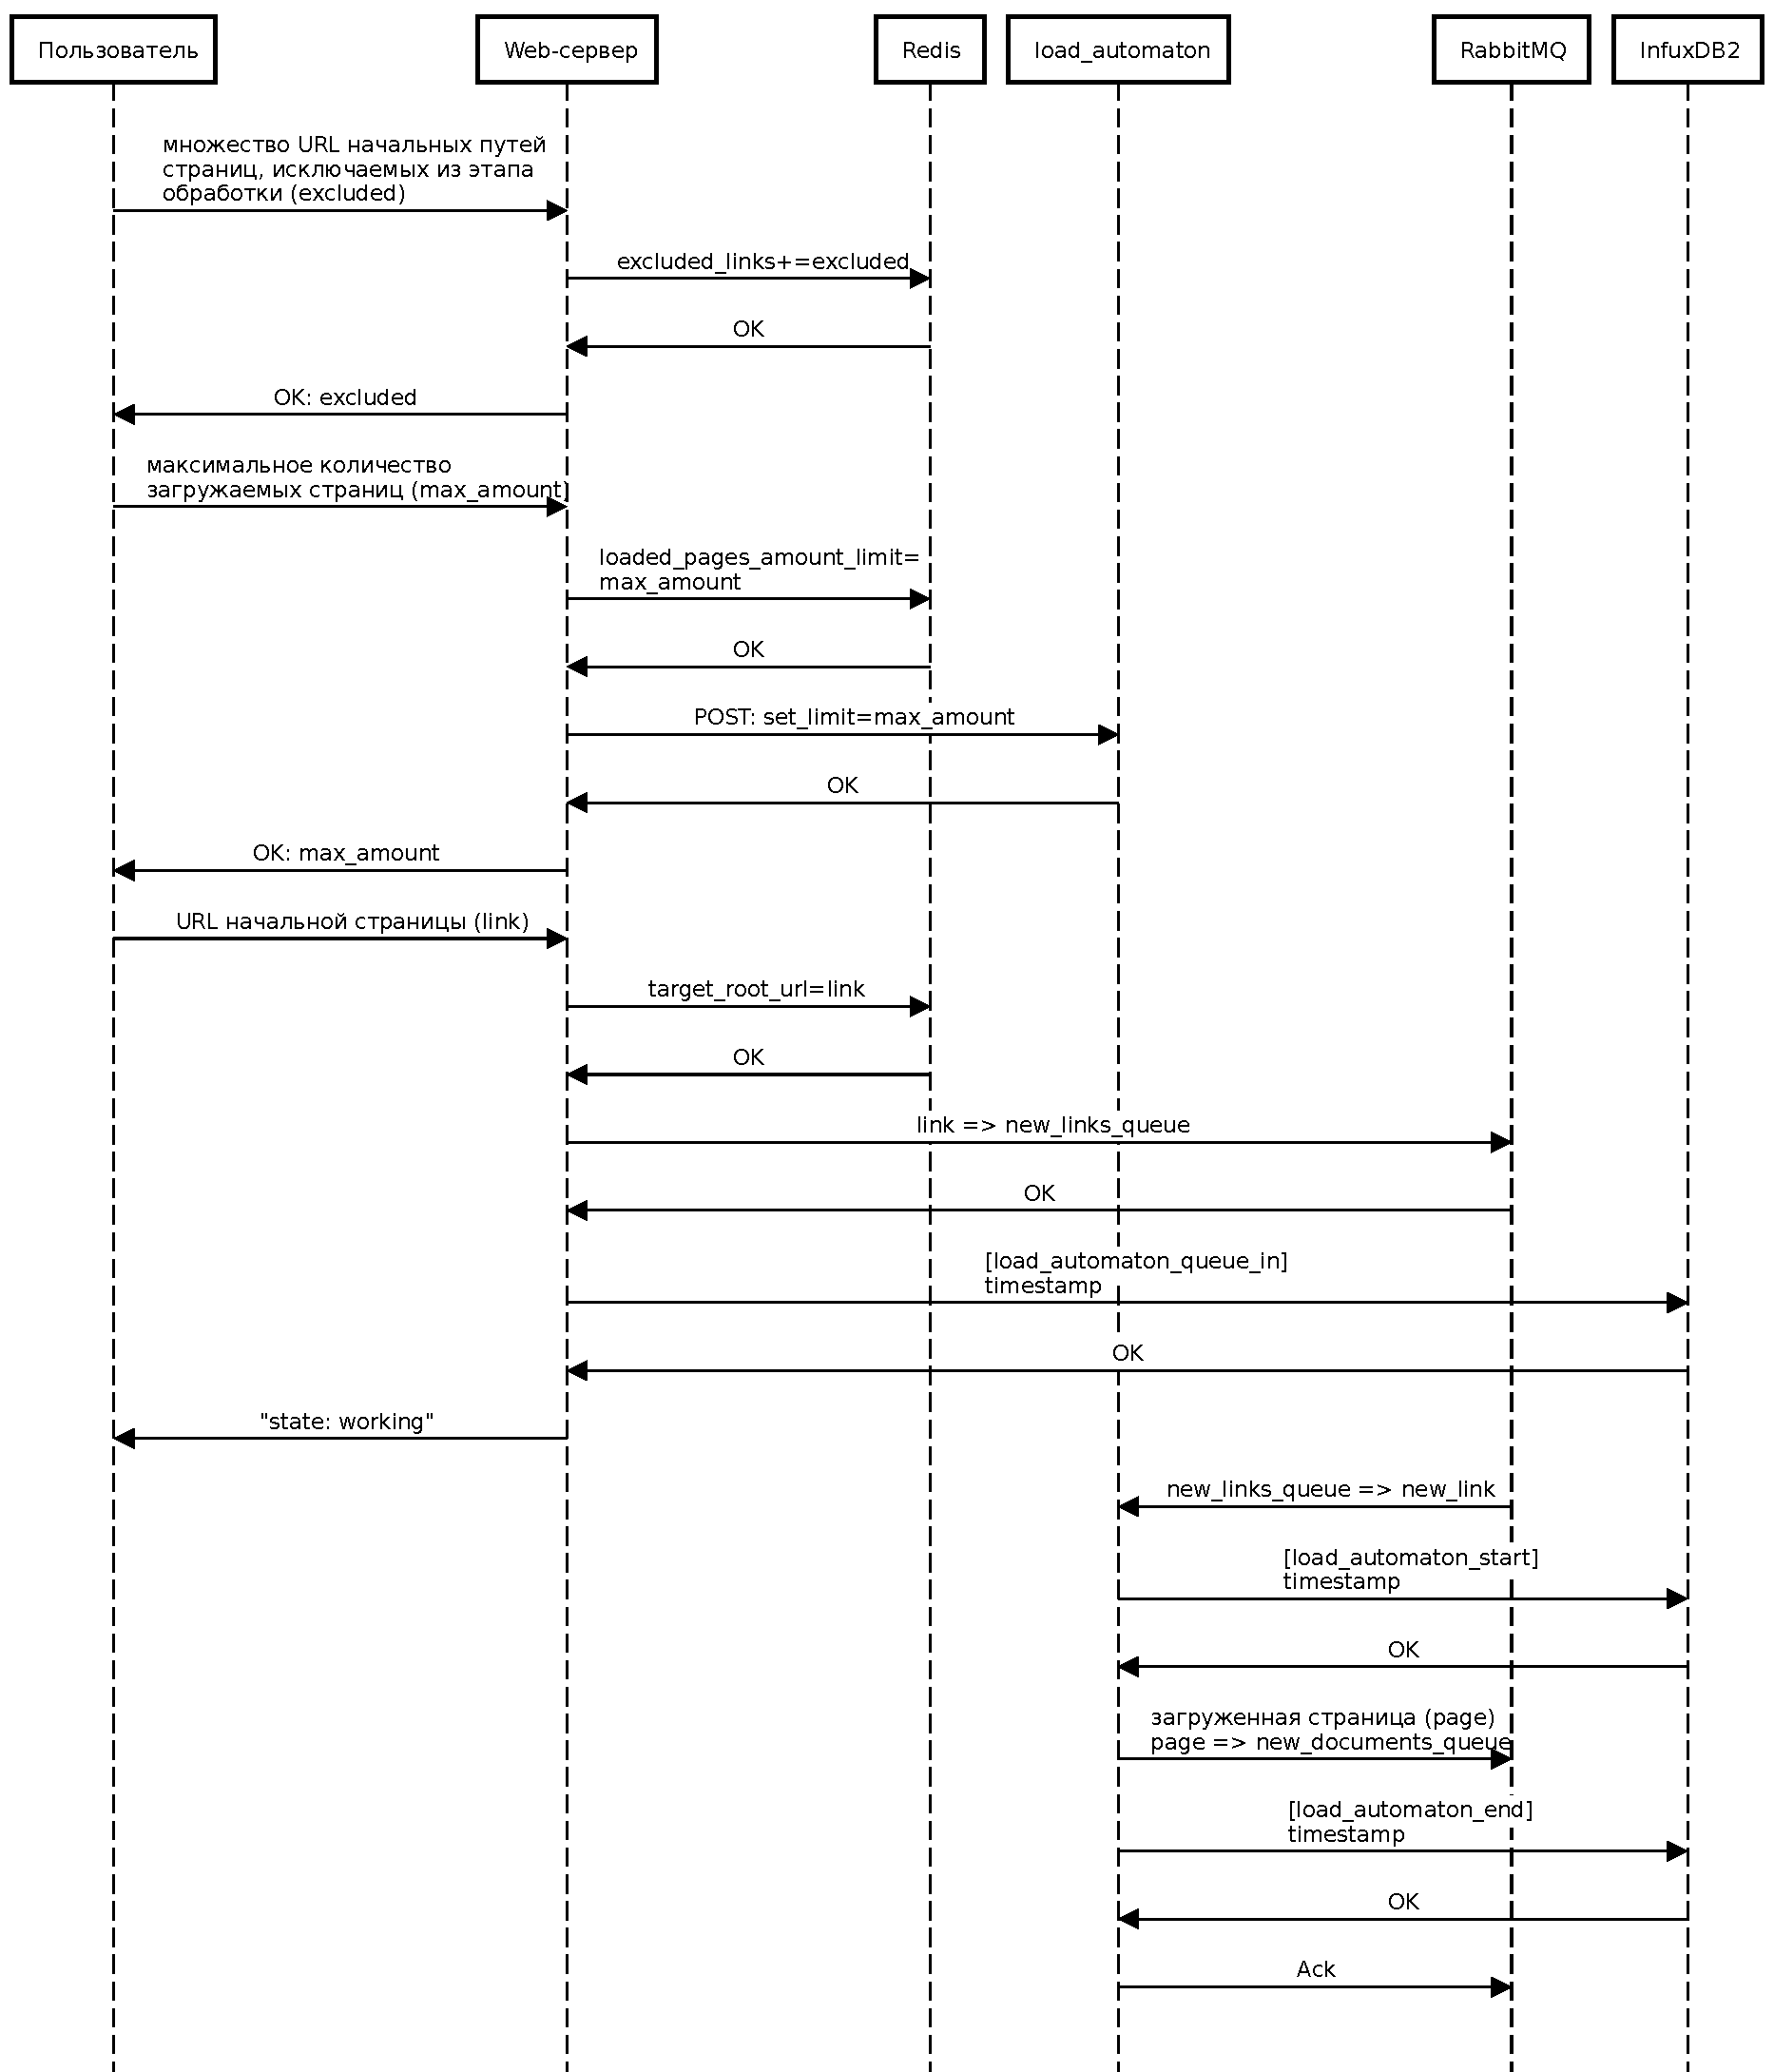
\includegraphics[width=1\linewidth]{inc/img/sequence_diagram_pt_1.pdf}}
	\caption{Диаграмма последовательности --- Начало}
	\label{img:sequence-diagram-pt-1}
\end{figure}

\begin{figure}[!ht]
	\center{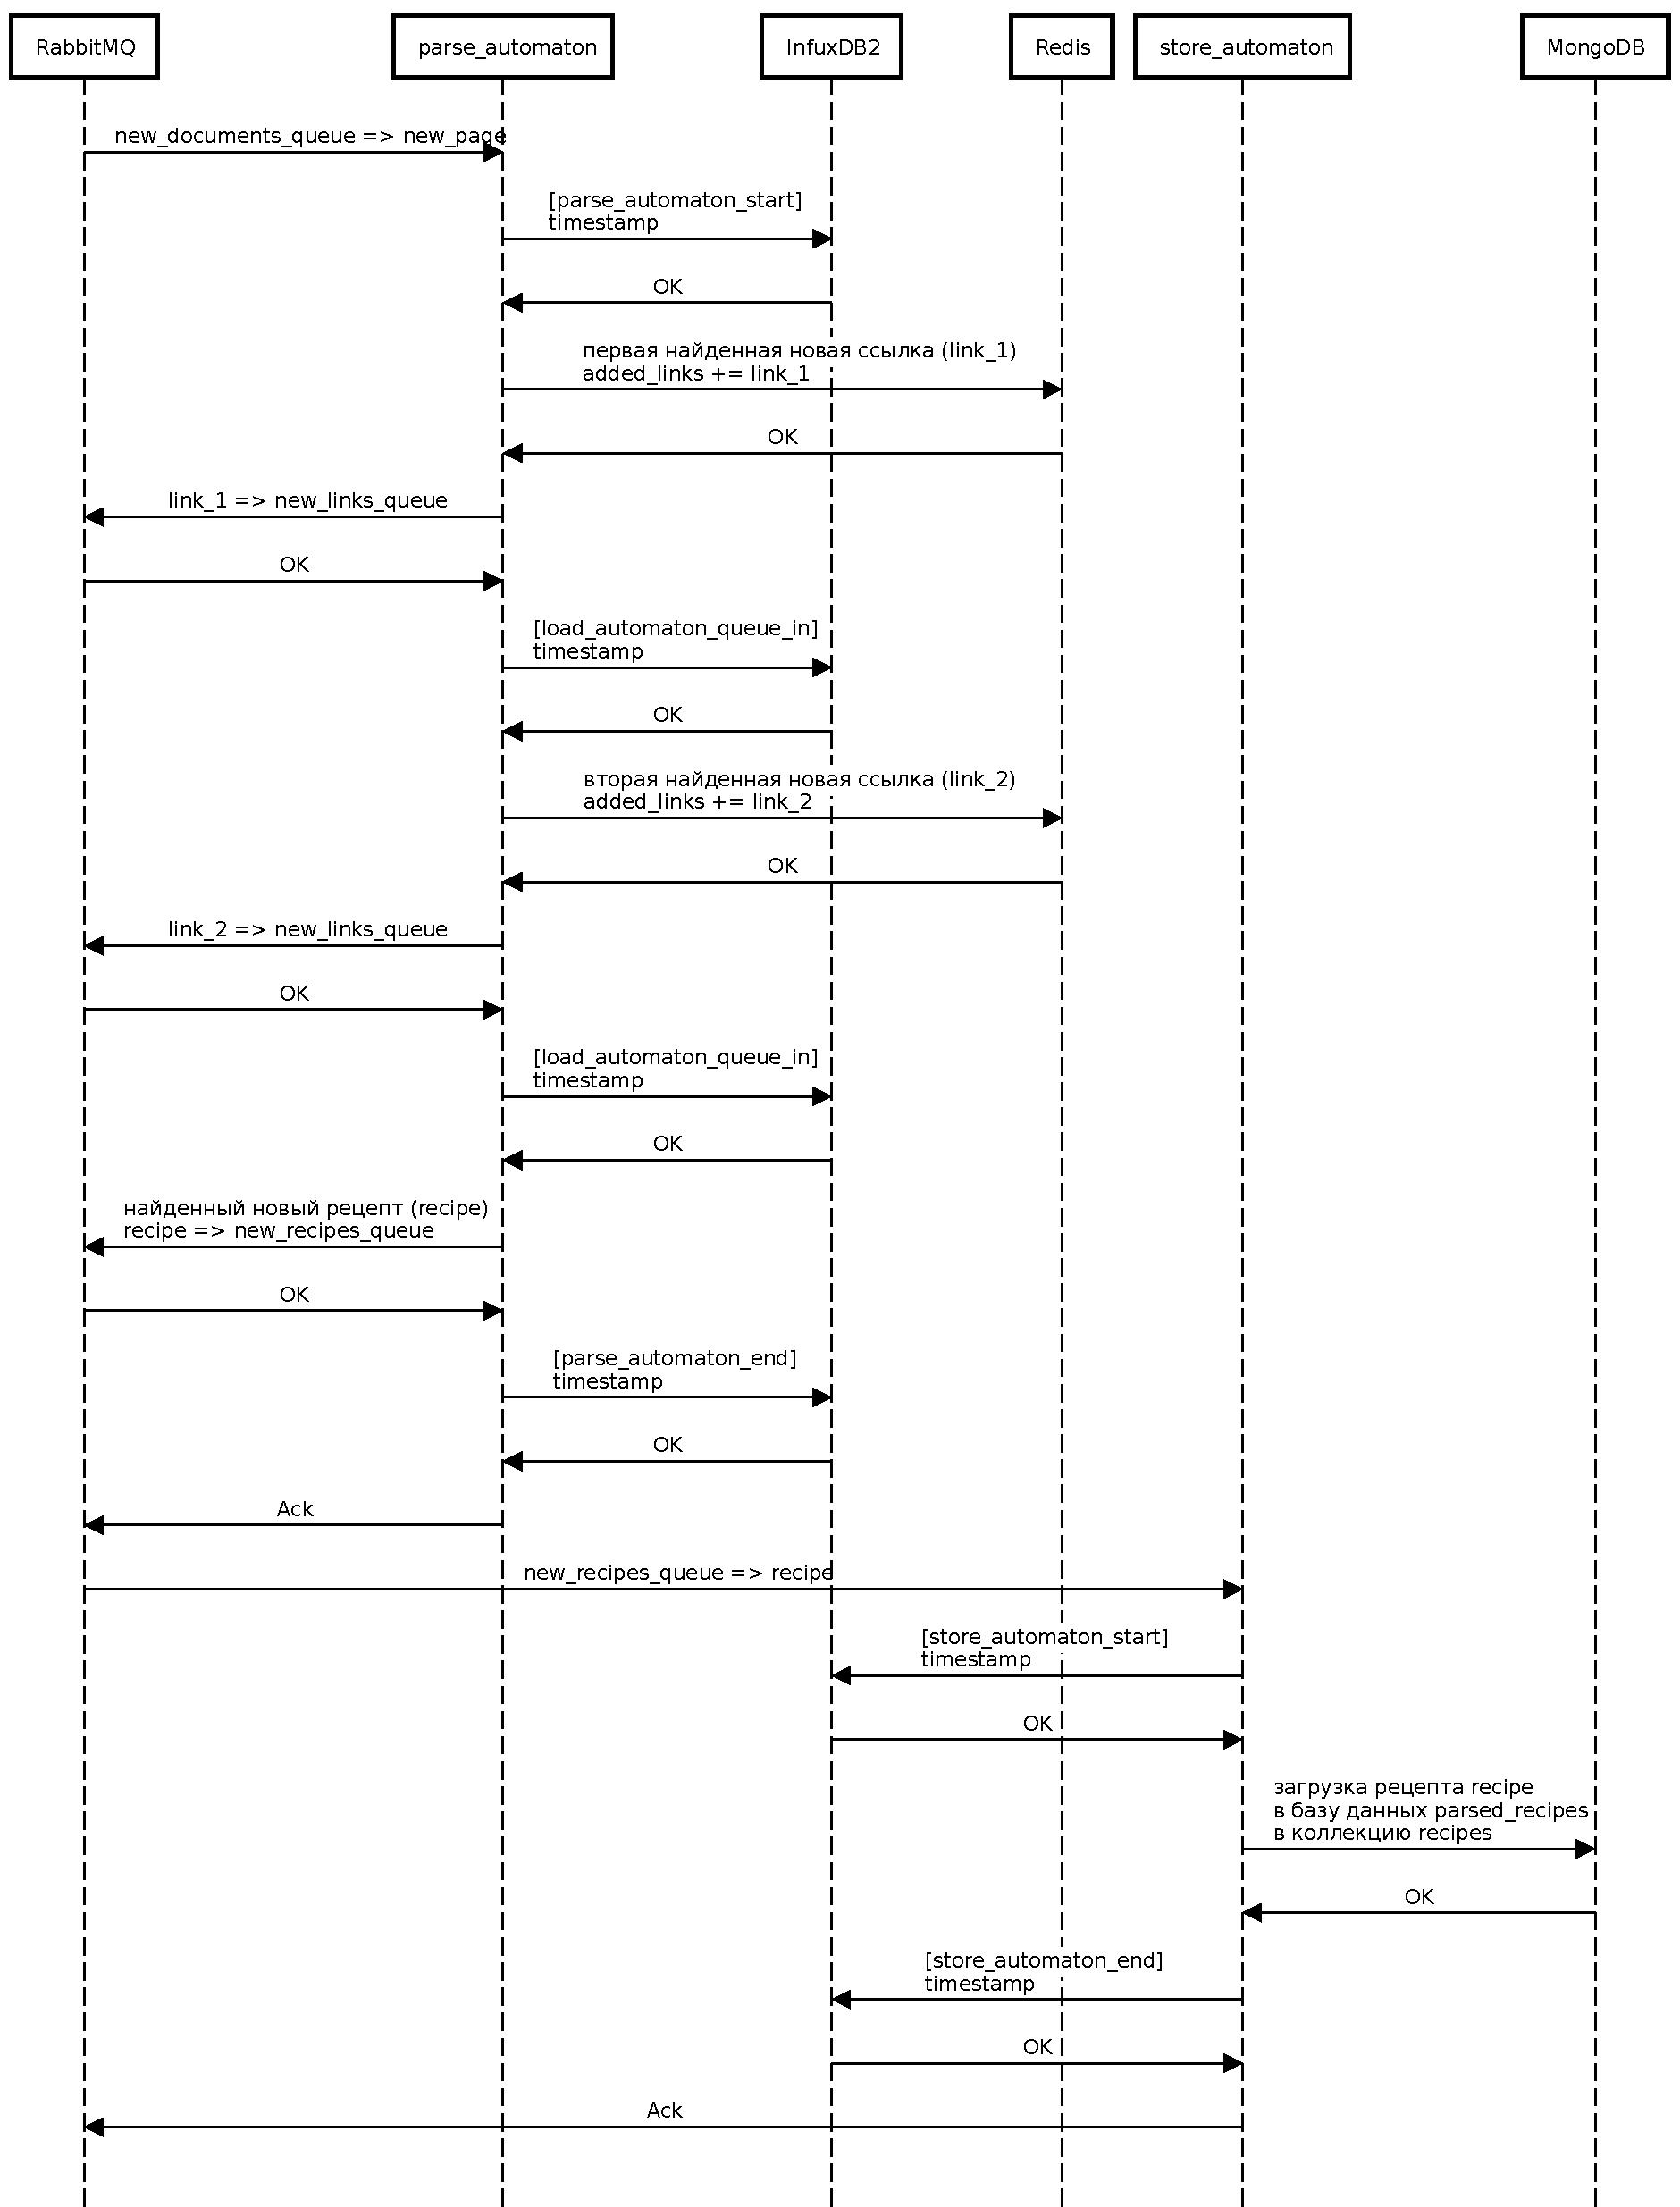
\includegraphics[width=1\linewidth]{inc/img/sequence_diagram_pt_2.pdf}}
	\caption{Диаграмма последовательности --- Конец}
	\label{img:sequence-diagram-pt-2}
\end{figure}

\clearpage

\aasection{Тестирование}{sec:tests}

В листинге~\ref{lst:test-html} представлен содержащий рецепт $HTML$-файл, на котором проводилось тестирование.

\begin{code}
	\captionof{listing}{Тестовый $HTML$-файл. Многоточием обозначен несущественный текст}
	\label{lst:test-html}
	\begin{minted}
		[
		frame=single,
		framesep=2mm,
		baselinestretch=1.2,
		fontsize=\scriptsize,
		]{text}
...
<h2 class="ny__set__title">
Гриль-чиз с луковым джемом </h2>
</div>
...
<div class="ny__details-container__root h2">
<div class="ny__dish-details__title-content__container">
<h1 itemprop="name" class="ny__details-subtitle__root">
Гриль-чиз с луковым джемом </h1>
</div>
...
<div class="ny__dish-details__content-root">
<div class="ny__dish-details__left-side">
<div class="ny__details-container__root content">
<p class="ny__details-subtitle__root"> В наборе</p></br>
<p class="ny__dishes-details__content" itemprop="recipeInstructions">тостовый хлеб, соус
бешамель, сыр моцарелла, луковый джем</p></br>
<p class="ny__details-subtitle__root">На вашей кухне</p>
<ul></br>
</ul></br>
<p class="ny__dishes-details__content" itemprop="recipeInstructions">* <img
src="/recipes/images/icons/board.png" width="16" /> <b>доска</b></p></br>
<p class="ny__details-subtitle__root"> Как готовить</p></br>
<p class="ny__dishes-details__content" itemprop="recipeInstructions">Включаем духовку на
**200°С** (режим верх-низ)</p></br>
<hr></br>
<p class="ny__dishes-details__content" itemprop="recipeInstructions">Ломтики тостового
хлеба кладем на противень</p></br>
<hr></br>
<p class="ny__dishes-details__content" itemprop="recipeInstructions">Соусом бешамель
смазываем <b>хлеб</b></p></br>
<p class="ny__dishes-details__content" itemprop="recipeInstructions">Луковый джем
равномерно выкладываем на <b>соус</b></p></br>
<p class="ny__dishes-details__content" itemprop="recipeInstructions">Сыр моцарелла
раскладываем сверху</p></br>
<hr></br>
<p class="ny__dishes-details__content" itemprop="recipeInstructions">Отправляем в
духовку на <img src="/recipes/images/icons/time.png" width="16" /> <b>10 минут</b>
</p></br>
<hr></br>
<p class="ny__dishes-details__content" itemprop="recipeInstructions">Разрезаем пополам
наискосок и кладем на тарелку</p></br>
<hr></br>
**Если нет духовки, рецепт для сковороды <img src="/recipes/images/icons/pan.png"
width="16" /> можно посмотреть по QR коду на пакете блюда</br>
<p class="ny__dishes-details__content" itemprop="recipeInstructions">или титульном
листе**</p></br>
<hr>
<p class="ny__dishes-details__content" itemprop="recipeInstructions">Корректируйте время
приготовления в соответствии с вашей кухонной техникой</p></br>
...
	\end{minted}
\end{code}

В листинге~\ref{lst:test-recipe} представлен результат работы приложения на тестовых данных.
\begin{code}
	\captionof{listing}{Полученный рецепт в формате $JSON$}
	\label{lst:test-recipe}
	\begin{minted}
		[
		frame=single,
		framesep=2mm,
		baselinestretch=1.2,
		fontsize=\scriptsize,
		]{text}
{
	"_id": {
		"$oid": "673fe6706267963c9f480bbf"
	},
	"id": {
		"$numberLong": "1732241008828292228"
	},
	"issue_id": {
		"$numberLong": "9038"
	},
	"url": "https://elementaree.ru/gril-ciz",
	"title": "Гриль-чиз с луковым джемом",
	"ingredients": [
	{
		"unit": "none",
		"amount": "none",
		"name": "В наборе"
	},
	{
		"name": "тостовый хлеб",
		"amount": "none",
		"unit": "none"
	},
	{
		"unit": "none",
		"name": "соус бешамель",
		"amount": "none"
	},
	{
		"name": "сыр моцарелла",
		"unit": "none",
		"amount": "none"
	},
	{
		"name": "луковый джем",
		"unit": "none",
		"amount": "none"
	}
	],
	"steps": [
	"Включаем духовку на 200°С (режим верх-низ)",
	"Ломтики тостового хлеба кладем на противень",
	"Соусом бешамель смазываем хлеб",
	"Луковый джем равномерно выкладываем на соус",
	"Сыр моцарелла раскладываем сверху",
	"Отправляем в духовку на 10 минут",
	"Разрезаем пополам наискосок и кладем на тарелку или титульном листе**"
	],
	"image_url": "https://static.elementaree.ru/003241/thumb_m/21fe2f0e0e8e3a6685027e7931e8733e.jpg"
}
	\end{minted}
\end{code}

\clearpage

\aasection{Описание исследования}{sec:study}

В ходе исследования требуется сформировать лог обработки задач, найти среднее время обработки задачи в каждом обслуживающем аппарате, среднее время ожидания в каждой очереди, среднее время существования задачи, расчёт среднего времени учитывает только задачи, прошедшие через все обслуживающие аппараты.

Для формирования результирующих данных в $Grafana$ были созданы информационные панели, пример которых приведён на рисунке~\ref{img:dashboard}.

В таблице~\ref{tab:queue-wait} отображено среднее время ожидания задач в очередях. Видно, что среднее время ожидания задач в очереди новых ссылок на 5 порядков больше по сравнению с остальными очередями.

\begin{table}[!ht]
	\centering
	\caption{Среднее время ожидания задач в очередях}
	\label{tab:queue-wait}
	\begin{tabular}{|c|r|}
		\hline
		\textbf{}                       & \multicolumn{1}{c|}{\textbf{Среднее время ожидания, мс}} \\ \hline
		\textbf{Очередь новых ссылок}   & 187536                                                   \\ \hline
		\textbf{Очередь новых страниц}  & 4,96                                                     \\ \hline
		\textbf{Очередь новых рецептов} & 9,87                                                     \\ \hline
	\end{tabular}
\end{table}

В таблице~\ref{tab:automaton-processing} отображено среднее время обработки задач обслуживающими аппаратами. Видно, что среднее время обработки обслуживающим аппаратом, загружающим страницы всего на 2--3 порядка больше по сравнению с остальными аппаратами, а наименьшее количество времени занимает сохранение рецепта в базу данных новых рецептов.

\begin{table}[!ht]
	\centering
	\caption{Среднее время обработки задач обслуживающими аппаратами}
	\label{tab:automaton-processing}
	\begin{tabular}{|c|r|}
		\hline
		\textbf{}                & \multicolumn{1}{c|}{\textbf{Среднее время обработки, мс}} \\ \hline
		\textbf{load\_automaton}  & 1672                                                      \\ \hline
		\textbf{parse\_automaton} & 71,6                                                      \\ \hline
		\textbf{store\_automaton} & 3,18                                                      \\ \hline
	\end{tabular}
\end{table}

В таблице~\ref{tbl:b_log} приведен фрагмент лога обработки. Обозначения событий:
\begin{itemize}
    \item la\_queue\_in --- поступление задачи в очередь $new\_links\_queue$;
    \item la\_start --- начало обработки задачи $load\_automaton$;
    \item la\_end — окончание обработки задачи $load\_automaton$;
    \item pa\_start --- начало обработки задачи $parse\_automaton$;
    \item pa\_end — окончание обработки задачи $parse\_automaton$;
    \item sa\_start --- начало обработки задачи $store\_automaton$;
    \item sa\_end — окончание обработки задачи $store\_automaton$.
\end{itemize}

\begin{longtable}{|p{.33\textwidth - 2\tabcolsep}|p{.33\textwidth - 2\tabcolsep}|p{.33\textwidth - 2\tabcolsep}|}
    \caption{Фрагмент лога обработки (начало)}\label{tbl:b_log}
    \\
    \hline
    Метка времени, мкс & Событие             & ID записи \\
    \hline
    \endfirsthead
    \caption{Фрагмент лога обработки (окончание)}
    \\
    \hline
    Метка времени, мкс   & Событие    & ID записи     \\
    \hline
    \endhead
    \hline
    \endfoot
    \endlastfoot
    \hline
    1731879526380238300 & la\_queue\_in & 1731879526378991099\\ \hline
    1731879526393213700 & la\_start & 1731879526378991099\\ \hline
    1731879527114415900 & la\_end & 1731879526378991099\\ \hline
    1731879527128372200 & pa\_start & 1731879526378991099\\ \hline
    1731879527262992000 & la\_queue\_in & 1731879527262313032\\ \hline
    1731879527265691000 & la\_queue\_in & 1731879527265136152\\ \hline
    1731879527266213000 & la\_start & 1731879527262313032\\ \hline
    1731879527268402000 & la\_queue\_in & 1731879527267816238\\ \hline
    1731879527271080000 & la\_queue\_in & 1731879527270563999\\ \hline
    1731879527273238800 & la\_queue\_in & 1731879527272774193\\ \hline
    1731879527275623700 & la\_queue\_in & 1731879527275098647\\ \hline
    1731879527277794300 & la\_queue\_in & 1731879527277385178\\ \hline
    1731879527280386000 & la\_queue\_in & 1731879527279724089\\ \hline
    1731879527282905300 & la\_queue\_in & 1731879527282345508\\ \hline
    1731879527285488400 & la\_queue\_in & 1731879527284825708\\ \hline
    1731879527287928800 & la\_queue\_in & 1731879527287471991\\ \hline
    1731879527290059000 & la\_queue\_in & 1731879527289660254\\ \hline
    1731879527292314400 & la\_queue\_in & 1731879527291868493\\ \hline
    1731879527294487600 & la\_queue\_in & 1731879527294055989\\ \hline
    1731879527297173500 & la\_queue\_in & 1731879527296607985\\ \hline
    1731879527299707400 & la\_queue\_in & 1731879527299173741\\ \hline
    1731879527302084900 & la\_queue\_in & 1731879527301598976\\ \hline
    1731879527304585500 & la\_queue\_in & 1731879527304039366\\ \hline
    1731879527306922000 & la\_queue\_in & 1731879527306499173\\ \hline
    1731879527308988700 & la\_queue\_in & 1731879527308584212\\ \hline
    1731879527311350500 & la\_queue\_in & 1731879527310899517\\ \hline
    1731879527314368800 & la\_queue\_in & 1731879527313698192\\ \hline
    1731879527317367000 & la\_queue\_in & 1731879527316716728\\ \hline
    1731879527320028200 & la\_queue\_in & 1731879527319516382\\ \hline
    1731879527322356000 & la\_queue\_in & 1731879527321835877\\ \hline
\end{longtable}

По результатам проведенного исследования сделан вывод о том, что события лога упорядочены по возрастанию временных меток, а также о том, что, несмотря на более долгий процесс загрузки отдельной страницы, решающим фактором, влияющим на скорость работы системы в целом является большое количество новых ссылок, подлежащих загрузке. Для увеличения производительности работы приложения следует увеличить количество рабочих потоков в обслуживающем аппарате, загружающем страницы и/или создать несколько экземпляров данного сервиса.

\aaunnumberedsection{ЗАКЛЮЧЕНИЕ}{sec:outro}

Цель работы достигнута. Решены все поставленные задачи: 
\begin{itemize}
    \item анализ предметной области;
    \item разработка алгоритма обработки данных;
    \item создание ПО, реализующего разработанный алгоритм;
    \item исследование характеристик созданного ПО.
\end{itemize}
